%%%%%%%%%%%%%%%%%%%%%%%%%%%%%%%%%%%%%%%%%
% Thin Sectioned Essay
% LaTeX Template
% Version 1.0 (3/8/13)
%
% This template has been downloaded from:
% http://www.LaTeXTemplates.com
%
% Original Author:
% Nicolas Diaz (nsdiaz@uc.cl) with extensive modifications by:
% Vel (vel@latextemplates.com)
%
% License:
% CC BY-NC-SA 3.0 (http://creativecommons.org/licenses/by-nc-sa/3.0/)
%
%%%%%%%%%%%%%%%%%%%%%%%%%%%%%%%%%%%%%%%%%

%----------------------------------------------------------------------------------------
%	PACKAGES AND OTHER DOCUMENT CONFIGURATIONS
%----------------------------------------------------------------------------------------

\documentclass[a4paper, 11pt]{article} % Font size (can be 10pt, 11pt or 12pt) and paper size (remove a4paper for US letter paper)

\usepackage[protrusion=true,expansion=true]{microtype} % Better typography
\usepackage{graphicx} % Required for including pictures
\usepackage{wrapfig} % Allows in-line images
\usepackage{amsmath}
\usepackage{amsbsy}
\usepackage{amsthm}
\usepackage{mathpazo} % Use the Palatino font
\usepackage[T1]{fontenc} % Required for accented characters
\linespread{1.05} % Change line spacing here, Palatino benefits from a slight increase by default
\newcommand{\LL}{\mathcal{L}}
\newcommand{\q}{\tilde{q}}
\newcommand{\x}{\tilde{x}}
%\makeatletter
%\renewcommand\@biblabel[1]{\textbf{#1.}} % Change the square brackets for each bibliography item from '[1]' to '1.'
%\renewcommand{\@listI}{\itemsep=0pt} % Reduce the space between items in the itemize and enumerate environments and the bibliography
%
%\renewcommand{\maketitle}{ % Customize the title - do not edit title and author name here, see the TITLE block below
%\begin{flushright} % Right align
%{\LARGE\@title} % Increase the font size of the title
%
%\vspace{50pt} % Some vertical space between the title and author name
%
%{\large\@author} % Author name
%\\\@date % Date
%
%\vspace{40pt} % Some vertical space between the author block and abstract
%\end{flushright}
%}

%----------------------------------------------------------------------------------------
%	TITLE
%----------------------------------------------------------------------------------------

%\title{\textbf{Unnecessarily Long Essay Title}\\ % Title
%Focused and Deliciously Witty Subtitle} % Subtitle
%
%\author{\textsc{Ford Prefect} % Author
%\\{\textit{Interstellar University}}} % Institution
%
%\date{\today} % Date

%----------------------------------------------------------------------------------------

\begin{document}

%\maketitle % Print the title section

%----------------------------------------------------------------------------------------
%	ABSTRACT AND KEYWORDS
%----------------------------------------------------------------------------------------

%\renewcommand{\abstractname}{Summary} % Uncomment to change the name of the abstract to something else

%\begin{abstract}
%
%\end{abstract}
%
%\hspace*{3,6mm}\textit{Keywords:} lorem , ipsum , dolor , sit amet , lectus % Keywords
%
%\vspace{30pt} % Some vertical space between the abstract and first section

%----------------------------------------------------------------------------------------
%	ESSAY BODY
%----------------------------------------------------------------------------------------

%%%%%%% This part is wrong %%%%%%%%%%%%


%\section*{Introduction}
%The portrait of injection region is first discussed. It can be proved that it is impossible to change from holding to injection as the price increases. Then it is shown that it is impossible to always do nothing no matter how high the price is. At last, we prove that if we withdraw at one price which is above certain level, we will withdraw at any price that is larger than the price just mentioned.\\
%
%One important thing to remember is that if there is no difference between injection and holding, we will always hold. This is to say, at injecting point, injection is strictly better than holding.
%\section*{Injection region}
%First recall the HJB equation as following 
%\begin{equation*}
%\max(V_q-(e^x+\lambda), \LL V, -V_q +(e^x-\mu)) = 0
%\end{equation*}
%where 
%\begin{equation}\label{L}
%\LL V = \frac{1}{2}\sigma^2 V_{xx} + k(\alpha - x)V_x - \beta V.
%\end{equation}
%Next, we would like to use contradiction method to show that it is impossible to change from holding to injection as price increases. If not, let $(x_0,q_0)$ be the point of changing. 
%Then the smooth fit conditions show
%\begin{equation}\label{smooth}
%\begin{split}
%V(x_0-,q_0) & = V(x_0+,q_0)\\
%V_q(x_0-,q_0) &= V_q(x_0+,q_0) \\
%V_x(x_0-,q_0) &= V_x(x_0+,q_0)\\
%\exists V_{xx}(x_0+,q_0) &\mbox{ and } V_{xx}(x_0-,q_0).
%\end{split}
%\end{equation}\footnote{The right and left second order derivatives may not equal to each other but they both exsit. That is to say, the value function may not be second order continuous. However, the Ito's formula still holds because the Ito-Tanaka theorem shows that Ito's formula holds with countable discontinuous points.}
%Changing from holding to injection can be described as 
%\begin{equation}\label{changing}
%\begin{split}
%V_q(x_0+,q_0) &= e^{x_0} + \lambda\\
%\LL V_(x_0+,q_0) &<  0\\
%V_q(x_0+,q_0) &> e^{x_0} - \mu\\
%V_q(x_0-,q_0) & \leq e^{x_0}+\lambda\\
%\LL V_(x_0-,q_0) &= 0 \\
%V_q(x_0-,q_0) &> e^{x_0} - \mu.\\
%\end{split}
%\end{equation}\footnote{The second inequality must be strict because $(x_0,q_0)$ is an injecting point at which injection is strictly better than holding.}
%%It is necessary  to prove the second inequality can't be strict. If not 
%%\begin{equation}
%%\LL V_(x_0+,q_0) = 0 = \LL V_(x_0-,q_0)
%%\end{equation}
%%Noticing that $V(x_0-,q_0)  = V(x_0+,q_0)$ and $V_x(x_0-,q_0) &= V_x(x_0+,q_0)$,  $ V_{xx}(x_0+,q_0) =  V_{xx}(x_0-,q_0)$.
%Next we would like to prove that the injection point can't be isolated. If not we must have 
%\begin{equation*}
%\begin{split}
%\LL V(x,q_0) &= 0 \quad \forall x \in (x_0,+\infty)\cap\{\mbox{holding region}\}\\
%\LL V(x,q_0) &= 0 \quad \forall x \in (-\infty,x_0)\cap\{\mbox{holding region}\}.
%\end{split}
%\end{equation*}
%Noticing that the right and left second order derivatives of value function with respect to $x$ exists,
%\begin{equation*}
%\begin{split}
%\LL V(x_0+,q_0) &= \lim_{x \rightarrow x_0+} \LL V(x,q_0) = 0\\
%\LL V(x_0-,q_0) &= \lim_{x \rightarrow x_0-} \LL V(x,q_0) = 0.
%\end{split}
%\end{equation*}
%Therefore $\LL V(x_0,q_0) = 0$ which contradicts the fact that $(x_0,q_0)$ is an injection point. Together with smoothness, there must be a $x_1 > x_0$ such that we inject at any point belongs to the set $I = \{(x,q_0)| x \in [x_0,x_1)\}$.Therefore for any point in $I$
%\begin{equation*}
%\begin{split}
%V_q(x,q_0) &= e^{x} + \lambda\\
%\LL V_(x+,q_0) &<  0\\
%V_q(x,q_0) &> e^{x} - \mu.\\
%\end{split}
%\end{equation*}
%By the convexity for $V(x,q)$ with respect to $q$
%\begin{equation*}
%V_q(x,q) = e^{x} + \lambda \quad \forall (x,q) \in [x_0,x_1]\times [0,q_0].
%\end{equation*}
%Therefore, 
%\begin{equation}\label{Vvalue}
%V(x,q_0) = q_0(e^{x}+\lambda) + V(x,0).
%\end{equation}\footnote{$V(x,0)$ may not be $0$, since we can make money by buying low and selling high.}
%%Right now, we are able to show why the second inequality is strict in (\ref{changing}). If not, plug (\ref{Vvalue}) into $\LL V(x_0+,q_0) = 0$,
%%\begin{equation}
%%%\begin{split}
%%\frac{1}{2}\sigma^2(q_0e^{x_0} + V_{xx}(x_0+,0)) + k(\alpha -x_0)(q_0e^{x_0}+V_x(x_0,0)) - \beta(q_0(e^{x_0}+\lambda) + V(x_0,0) = 0
%%%\end{split}
%%\end{equation}
%%Taking $q_0$
%Similarly, holding point can't be isolated as well. There exists a $x_2<x_0$ such that we hold at any point belongs to the set $H = \{(x,q_0)| x \in (x_2,x_0)\}\footnote{The point$(x_0,q_0)$ is excluded from this set because it is actually an injection point.}$. Therefore for any point in $H$
%\begin{equation*} 
%\begin{split}
%V_q(x,q_0) &< e^{x} + \lambda\\
%\LL V_(x-,q_0) &=  0\\
%V_q(x,q_0) & > e^{x} - \mu.\\
%\end{split}
%\end{equation*}\footnote{The first inequality is not strict because it holds at point $(x_0,q_0)$ while the third inequality is always strict since all the points are in the interior of the completion set of withdrawing region.}
%Since HJB equation holds for every point, therefore 
%\begin{equation*}
%e^x - \mu \leq V_q(x,q) \leq e^x + \lambda.
%\end{equation*}
%Thus
%%Combined with the facts that $V_q(x,q_0) < e^{x} + \lambda$ and $V(x,q)$ is convex with respect to $q$,
%\begin{equation*}
%q_0(e^x-\mu) + V(x,0) \leq V(x,q_0) \leq q_0(e^x+\lambda) + V(x,0)
%\end{equation*}
%for any point in $H$.\\
%To simplify the equation, let 
%\begin{equation*}
%f(x) = V(x,q_0) - q_0(e^x+ \lambda) - V(x,0).
%\end{equation*}
%Then 
%\begin{equation*}
%	f(x) \left\{
%	\begin{array}{rrr}
%\leq &0 &x_2<x<x_0\\
%= &0 & x_0\leq x< x_1.
%\end{array}
%\right.
%\end{equation*}
%Therefore $x_0$ is the local maximum\footnote{Actually, it is the global maximum point} which means $f''(x_0-) \leq 0.$\footnote{It is obvious that $f''(x_0+) = 0$.} What's more, from the smooth fit condition (\ref{smooth})
%\begin{equation}\label{fvalue}
%\begin{split}
%f(x_0-) &= f(x_0+) = 0\\
%f'(x_0-) &= f'(x_0+) = 0.
%\end{split}
%\end{equation} 
%On the other hand, 
%\begin{equation*}
%V(x,q_0) =f(x) + q_0(e^x+\lambda) + V(x,0)
%\end{equation*}
%Plug this in $\LL V(x_0+,q_0)< 0$ and $\LL V(x_0-,q_0) =0$
%\begin{equation*}
%\begin{split}
%\frac{1}{2}\sigma^2 f''(x_0+) + k(\alpha - x_0)f'(x_0) - \beta f(x_0) < -\frac{1}{2}\sigma^2 q_0 e^x + k(x_0 - \alpha)q_0e^x + \beta q_0(e^x + \lambda) \\-\frac{1}{2}\sigma^2 V_{xx}(x_0+,0) - k (\alpha -x_0) V_x(x_0,0) + \beta V(x_0,0)
%\end{split}
%\end{equation*}
%and
%\begin{equation*}
%\begin{split}
%\frac{1}{2}\sigma^2 f''(x_0-) + k(\alpha - x_0)f'(x_0) - \beta f(x_0) = -\frac{1}{2}\sigma^2 q_0 e^x + k(x_0 - \alpha)q_0e^x + \beta q_0(e^x + \lambda) \\-\frac{1}{2}\sigma^2 V_{xx}(x_0-,0) - k (\alpha -x_0) V_x(x_0,0) +\beta V(x_0,0).
%\end{split}
%\end{equation*}
%Substitute (\ref{fvalue}) and $f''(x_0+) = 0$ into the previous two formulas we have
%\begin{equation*}
%\begin{split}
%0<-\frac{1}{2}\sigma^2 q_0 e^x + k(x_0 - \alpha)q_0e^x + \beta q_0(e^x + \lambda) \\-\frac{1}{2}\sigma^2 V_{xx}(x_0+,0) - k (\alpha -x_0) V_x(x_0,0) + \beta V(x_0,0)
%\end{split}
%\end{equation*}
%and
%\begin{equation*}
%\begin{split}
%\frac{1}{2}\sigma^2 f''(x_0-) = -\frac{1}{2}\sigma^2 q_0 e^x + k(x_0 - \alpha)q_0e^x + \beta q_0(e^x + \lambda) \\   -\frac{1}{2}\sigma^2 V_{xx}(x_0-,0) - k (\alpha -x_0) V_x(x_0,0) + \beta V(x_0,0).
%\end{split}
%\end{equation*}
%However, $f''(x_0-)\leq 0$ thus if $V_{xx}(x_0+,0) = V_{xx}(x_0-,0)$ then there is a contradiction.\\
%If $V_{xx}(x_0+,0) \neq V_{xx}(x_0-,0)$ which means that $(x_0,0)$ is on the boundary of injection and holding, by the convexity of $V(x,q)$ with respect to $q$, all the points $\{(x_0,q), q\leq q_0\}$ are on the boundary. Define
%\begin{equation*}
%q_1 = \sup\{q\leq Q |(x_0,q) \mbox{ is on the boundary}\}.
%\end{equation*}
%By definition, $q_0 \leq q_1 \leq Q$. Moreover, $\LL V(x_0,q_1) = 0$. If not, by the continuity of $V_{xx}, V_x$ and $V$ with respect to $q$, we can have a $q_2 > q_1$ such that $(x_0,q_2)$ is on the boundary which contradicts the definition of $q_1$.  Noticing that $\forall q<q_1$
%\begin{equation*}
%\LL V(x_0+,q) = \frac{1}{2}\sigma^2(qe^{x_0} + V_{xx}(x_0+,0)) + k(\alpha -x_0)(qe^{x_0}+V_x(x_0,0)) - \beta(q(e^{x_0}+\lambda) + V(x_0,0)).
%\end{equation*}
%Take $q \rightarrow q_1$,
%\begin{equation*}
%0 = \LL V(x_0+,q_1) = \frac{1}{2}\sigma^2(q_1e^{x_0} + V_{xx}(x_0+,0)) + k(\alpha -x_0)(q_1e^{x_0}+V_x(x_0,0)) - \beta(q_1(e^{x_0}+\lambda) + V(x_0,0)).
%\end{equation*}
%On the other hand $\forall q<q_1$
%\begin{equation*}
%\LL V(x_0-,q) = \frac{1}{2}\sigma^2(qe^{x_0} + V_{xx}(x_0-,0)) + k(\alpha -x_0)(qe^{x_0}+V_x(x_0,0)) - \beta(q(e^{x_0}+\lambda) + V(x_0,0)).
%\end{equation*}
%Take $q \rightarrow q_1$,
%\begin{equation*}
%0 = \LL V(x_0-,q_1) = \frac{1}{2}\sigma^2(q_1e^{x_0} + V_{xx}(x_0-,0)) + k(\alpha -x_0)(q_1e^{x_0}+V_x(x_0,0)) - \beta(q_1(e^{x_0}+\lambda) + V(x_0,0)).
%\end{equation*}
%Thus $V_{xx}(x_0 + ,0) = V_{xx}(x_0-,0)$ which is a contradiction. All in all, we have proved that it is impossible to approach injecting region from below.

\section{Model}

Let $S_t$ be the price and its evolution follows 

\begin{equation}
  dS_t = \kappa(\gamma-\log(S_t))S_t dt + \sigma S_t dZ_t.
\end{equation}

Take $X_t = \log(S_t)$, by Ito's formula,

\begin{equation}
  dX_t = \kappa(\alpha - X_t) dt + \sigma dZ_t,
\end{equation}

where $\alpha = \gamma - \frac{\sigma^2}{2\kappa}$.\\ 

Let $Q_t \in [Q_{\min},Q_{\max}]$ denote the total amount of commodity in the storage facility at time $t$ where $Q_{\min},Q_{\max}$ are the minimum and maximum capacity. Here for simplicity, take them as $0$ and $100$ separately. \\

The decisions that a facility manager can make is when and how much shall be injected and withdraw from the facility. Denote cumulative amounts of commodity purchased and sold up to time $t$ as $L_t$ and $U_t$, respectively. Here and after, buy and inject have the same meaning, so do sell and withdraw. Then 

\begin{equation}
  dQ_t = dL_t - dU_t.
\end{equation}

An admissible control policy is a pair $(L_t,U_t)$ such that $Q_t \in [Q_{\min},Q_{\max}]$ for all $t$. $\mathcal{U}$ is used to denote all admissible policies.\\

Both injection and withdraw generate costs. Let $\lambda(q)dq$ be the cost of injecting $dq$ unit when the storage has $q$ unit already and $\mu(q)dq$ of withdrawing. We assume that $\lambda(q)$ and $\mu(q)$ are continuous. It is often easier to inject when empty and to withdraw when full. Therefore we assume that $\lambda(q)$ is increasing with respect to $q$ while $\mu(q)$ is decreasing. However, it is worth to note that \textbf{the monotonicity is not required for proof}.\\

The objective is to maximize discounted infinite-horizon discounted cash flows. Taking a discount factor $\beta \in (0,1)$, 

\begin{equation}
  V(x,q) = \max_{(L,U) \in \mathcal{U}} \mathbb{E}_{x,q} \left(\int_{0}^{\infty} e^{-\beta t}(e^{X_t} - \mu(Q^1_t))dU_t - \int_{0}^{\infty}e^{-\beta t}(e^{X_t} + \lambda(Q^2_t))dL_t\right)
\end{equation}

where $X_0 =x$ and $Q_0 = q$. What's more,
\begin{equation}
  \mu(Q^1_t) = \frac{1}{U_t - U_{t-}}\int_{U_{t-}}^{U_t} \mu(q) dq
\end{equation}

\begin{equation}
  \lambda(Q^2_t) = \frac{1}{L_t - L_{t-}}\int_{L_{t-}}^{L_t} \lambda(q) dq.
\end{equation}


 Since $V(x,q)$ is the maximum value that a facility manager can obtain from a storage facility, this is the value of the facility when the current spot price is $e^x$ and the amount is $q$.

\section{Intuition}

Since there are only two activities, buy and sell, the way of making a profit must be buy low and sell high. Actually, it is rigorously proved that the optimal policy must sell when price is high enough. However, the existence of transaction costs implies that the real buying price which includes injecting cost has a lower bound $\lambda(q)$. Therefore, the minimal selling price is $\lambda(q)+\mu(q)$. In this case, we may not buy at extremely low price because it takes a long time to go back to $\lambda(q)+\mu(q)$ level which means it may be impossible to make a profit resulting from discounting. This can be seen clearly when $\lambda(q)+\mu(q)$ is larger than the mean reverting level $\alpha$\footnote{Is there certain constraints guarantee the existence of lower bound of buying region?}. Here comes the difficulty of moving boundary method. \\

\textbf{No suitable initial guess for buying region exists. A initial guess needs to generated in the moving boundary method itself.}\\

What will the optimal strategy be without buying? It will be less aggressive because there is only one chance for selling. In other words, the selling price will be higher. On the other hand, the probability a buying strategy makes money depends on the selling strategy. The better selling strategy the larger probability certain buying strategy will make a profit. If a buying strategy can make money with the optimal selling strategy without buying, it must be able to make money with the optimal one with buying. Actually, the optimal selling strategy without buying is not necessary. All we need is a selling strategy that is less aggressive than the global optimal.\\

Here comes the method that overcome above difficulty.

\begin{enumerate}
  \item Assume there is no buying region at all while the selling strategy is selling all in stock at a super high price.
  \item Keep moving the selling boundary down to lower price until there appears a region that we can make a profit by buying.
\end{enumerate}

After the buying region is generated, it is quite natural to move the selling and buying boundary alternatively because the improvement of one has a positive effect on the other. Therefore the last step is 

\begin{enumerate}
 \item[3.] Move selling and buying boundaries alternatively until converges.
\end{enumerate}

The first two procedures are stage 1 while the last is stage 2. When we say move selling (or buying) boundary, it means that for each $q$, the price that generating the maximum selling (or buying) profit is moved to. In order to prove this method works, two things need to be done.

\begin{enumerate}
  \item Each time the boundary moves, the value function increases. Mathematically speaking, $V^{n+1} > V^{n}$.
  \item The moving conditions are always satisfied. This is to say, we can keep moving the boundary. Mathematically speaking, at both stages, $\left(-V_q^{n+1}(x,q) + (e^{x}-\mu(q))\right)_x <0$ at $n+1$ th selling boundary. At second stages, $\left(V_q^{n+1}(x,q) - (e^{x}+\lambda(q))\right)_x >0$ at $n+1$ th buying boundary.
\end{enumerate}



\section{Each time the boundary moves, the value function increases.}

Only consider the case that selling boundary is moved, because the other part is the same.\\


Denote $V^k(x,q)$ as the value function after nth moving boundary procedure and $S^k, B^k$ and $H^k$ are the buying, selling and holding region separately.\\

Assume at step $n+1$, the selling boundary is moved. This implies that $S^{n} \subset S^{n+1}$, $B^{n} = B^{n+1}$ and $H^{n} \supset H^{n+1}$ as shown in the figure. 

\begin{figure}[hbt]
  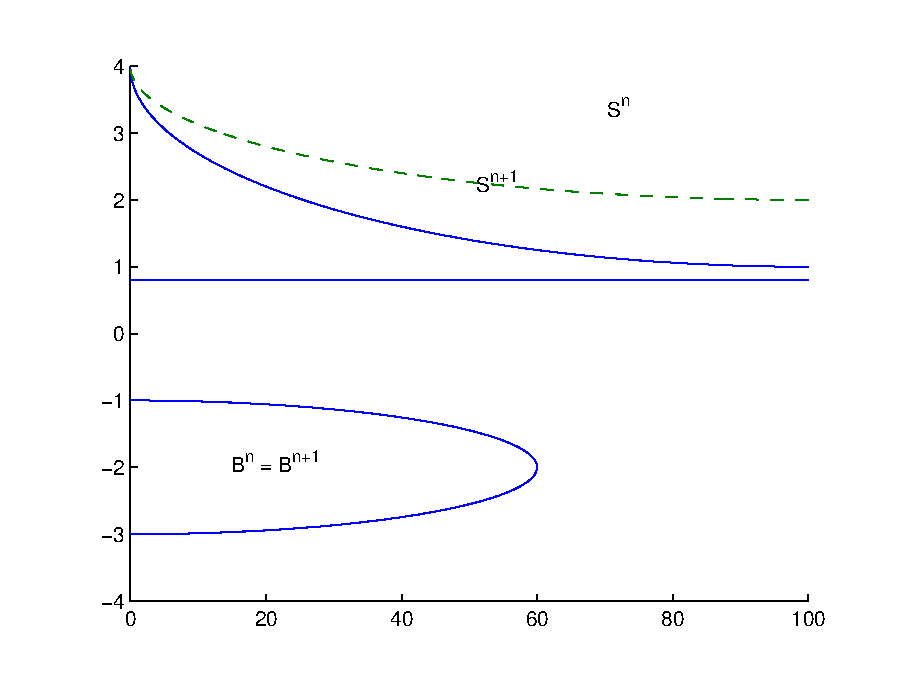
\includegraphics{SnSn+1Bn.eps}
  \caption{Regions of $S^n$, $S^{n+1}$ and $B^n = B^{n+1}$}
\end{figure}

Define $\Delta V^{n+1}(x,q) = V^{n+1}(x,q) - V^{n}(x,q)$. According to the conditions under which the selling boundary is moved, we have 

\begin{equation}\label{V}
\begin{split}
\Delta V_q^{n+1}(x,q) &= 0 \quad (x,q) \in S^{n}\\
\Delta V_q^{n+1}(x,q) &> 0 \quad (x,q) \in S^{n+1}/S^{n}\\
\LL \Delta V^{n+1}(x,q) &= 0 \quad (x,q) \in H^{n+1}\\
\Delta V_q^{n+1}(x,q) &= 0 \quad (x,q) \in B^{n} = B^{n+1}\\
\end{split}  
\end{equation}

\begin{figure}[hbt]\label{1ststage}
  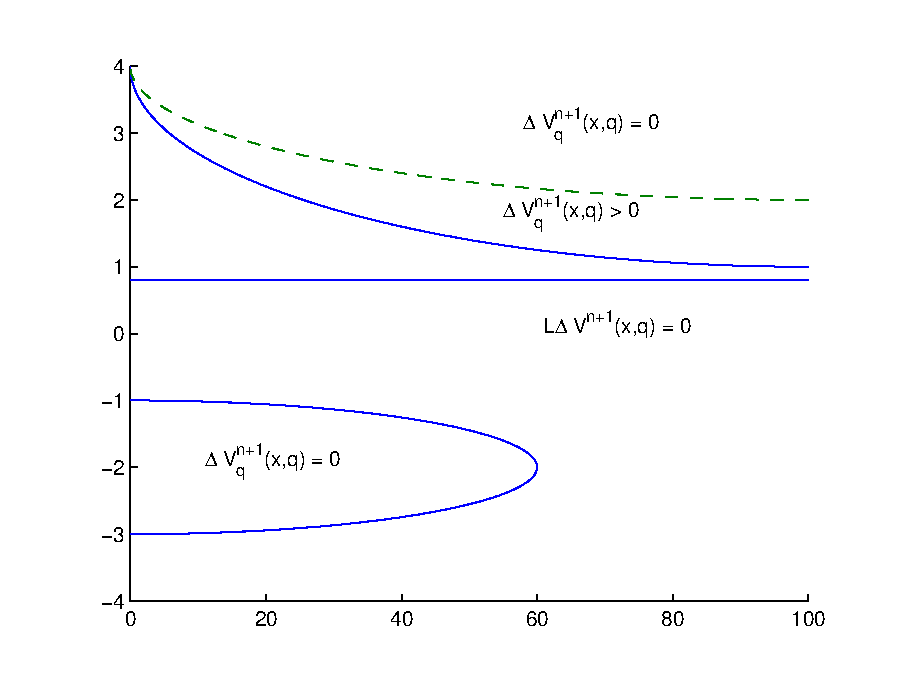
\includegraphics{deltaV.eps}
  \caption{The equations that $\Delta V^{n+1}$ satisfies.}
\end{figure}



Since $H^{n+1}$ doesn't have isolated vertical segment except $V_1 = \{(x,0)\in H^{n+1}\}$ and $V_2 = \{(x,100)\in H^{n+1}\}$, we can take derivative with respect to $q$ to the third equation.

\begin{equation}\label{Vq}
\begin{split}
\Delta V_q^{n+1}(x,q) &= 0 \quad (x,q) \in S^{n}\\
\Delta V_q^{n+1}(x,q) &> 0 \quad (x,q) \in S^{n+1}/S^{n}\\
\LL \Delta V_q^{n+1}(x,q) &= 0 \quad (x,q) \in H^{n+1}/(V_1 \cup V_2)\\
\Delta V_q^{n+1}(x,q) &= 0 \quad (x,q) \in B^{n} = B^{n+1}\\
\end{split}  
\end{equation}

Before moving any further, two properties of operator $\LL$ are needed. 

\begin{enumerate}
  \item It's impossible to have positive maximal interior point.
  \item It's impossible to have negative minimum interior point.
\end{enumerate}

\begin{proof}
Only the first one is proved, the second is the same.\\

If not, there exists $x$ which is the positive maximal interior point. Then $f'(x) = 0$ and $f''(x) \leq 0$. On the other hand, $\LL f(x) = 0$. By the definition of $\LL$,

\begin{equation}
\begin{split}
  &\frac{1}{2}\sigma^2 f'' + \kappa(\alpha - x) f' - \beta f = 0 \\
  \Rightarrow & 0<\beta f = \frac{1}{2}\sigma^2 f'' + \kappa(\alpha - x) f' \leq 0
\end{split}
\end{equation}

Contradiction!

\end{proof}

Here begins the proof of $\Delta V^{n+1}(x,0) \geq 0$.
\begin{proof}

Notice that with $q$ fixed, $f(x) = \Delta V_q^{n+1}(x,q)$ is the solution of $\LL f = 0$. Moreover, the boundary conditions are  $f(x_S)> 0$, where $(x_S,q) \in S^{n+1}/S^{n}$ and $f(x_B) = 0$, where $x_B$ is the largest $x$ satisfying $(x,q) \in B^{n} = B^{n+1}$.\\   

Therefore, by the two properties of $\LL$, $f(x)$ is non-negative for all points $(x,q) \in H^{n+1}$ and it achieves its maximum at point $x_S$. By the fact that $q$ is arbitrary, 
\begin{equation}
  \Delta V_q^{n+1}(x,q) \geq 0 \quad (x,q) \in H^{n+1}/(V_1 \cup V_2).
\end{equation}

Together with (\ref{Vq}), 

\begin{equation}\label{nonneg}
  \Delta V_q^{n+1}(x,q) \geq 0 \quad (x,q) \in \mathbb{R}\times[0,100]/(V_1 \cup V_2).
\end{equation}

There are two cases when the selling boundary moves.

\begin{enumerate}
  \item States of $q = 0$ is isolated.
  \item States of $q = 0$ is not isolated.
\end{enumerate}

\begin{figure}[hbt]
  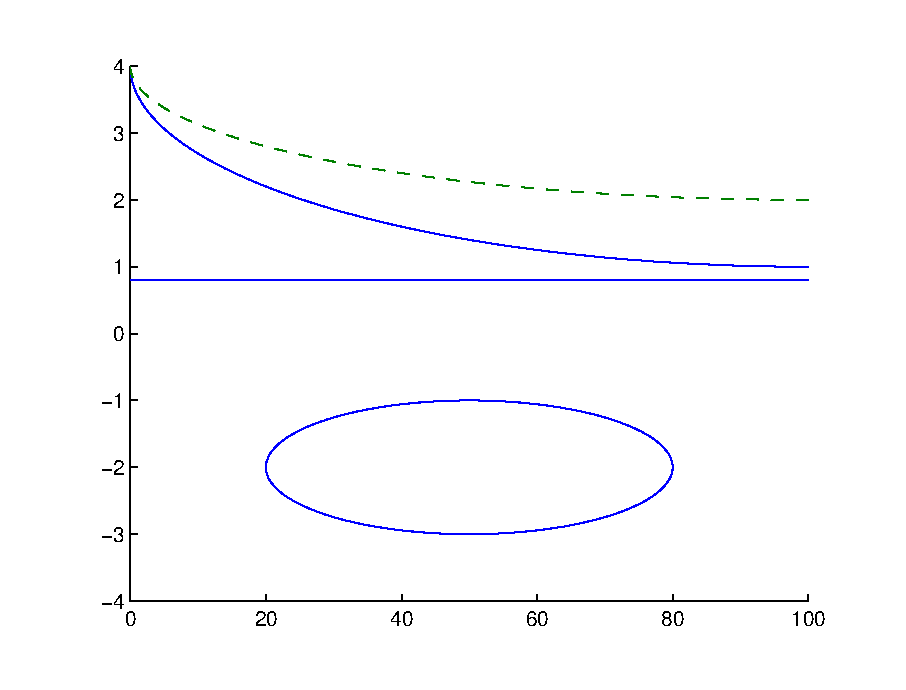
\includegraphics{Isolated.eps}
  \caption{When states of q = 0 is isolated when selling boundary moves.}
\end{figure}

\begin{figure}[hbt]
  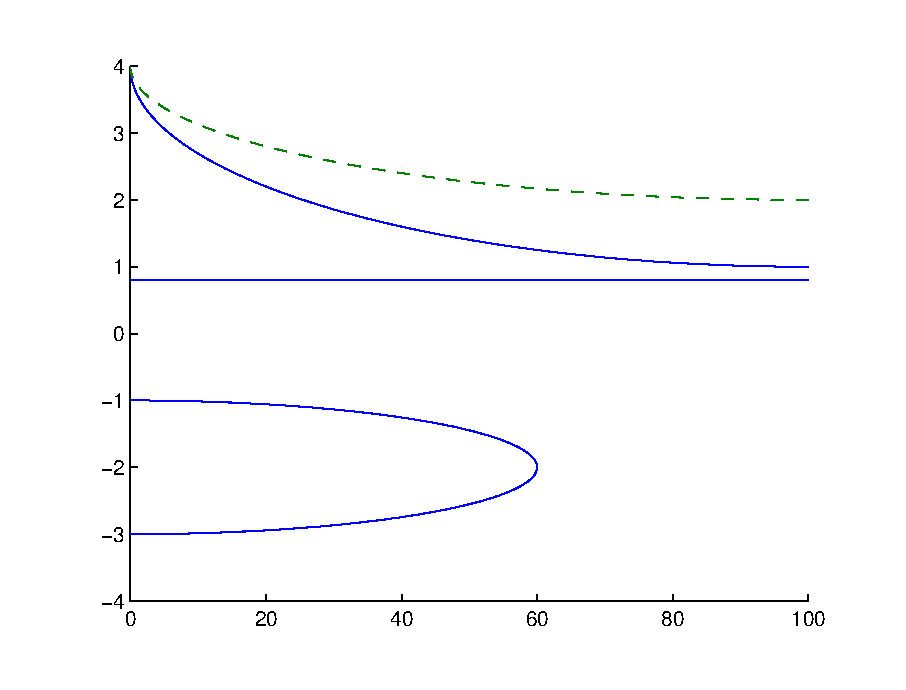
\includegraphics{NotIsolated.eps}
  \caption{When states q = 0 is not isolated when selling boundary moves.}
\end{figure}

In the first case, $\LL \Delta V^{n+1}(x,0) = 0 \quad \forall x \in \mathbb{R}$. By the fact that both $V^{n+1}$ and $V^{n}$ are bounded, $\Delta V^{n+1}(x,0)$ is also bounded. Combine these two we have $\Delta V^{n+1}(x,0) = 0 \quad \forall x \in \mathbb{R}$. What's more, (\ref{nonneg}) shows that 

\begin{equation}
  \Delta V^{n+1}(x,q) = \Delta V^{n+1}(x,0) + \int_{0}^{q} \Delta V_q^{n+1}(x,\tau)d\tau \geq 0+0 = 0.
\end{equation}


In the second case, we still want to show that $\LL \Delta V^{n+1}(x,0) = 0 \quad \forall x \in \mathbb{R}$. It is trivial when $(x,0) \in H^{n+1}$. To prove the case $(x,0) \notin H^{n+1}$, another assumption is needed. \\

\textbf{At a fixed level $x$, at most one of buying and selling happens which is the same as } 


\begin{equation}
\begin{split}
  (x,0) \notin H^{n+1} &\Leftrightarrow \text{Buying happens at level $x$} \\
  &\Leftrightarrow \text{(x,100) is not a selling point} \Leftrightarrow (x,100)\in H^{n+1}.
\end{split}
\end{equation}

Because for the optimal policy, it is proved at most one of buying and selling happens and both buying strategy and selling strategy is less aggressive than the optimal one. This assumption is reasonable. In the case $(x,0) \notin H^{n+1}$,

\begin{equation}\label{q100}
    \Delta V^{n+1}(x,0) = \Delta V^{n+1}(x,100) - \int_{0}^{100} \Delta V_q^{n+1}(x,q)dq.
\end{equation}

There are only two situations for $\{(x,q)| q \in (0,100)\}$,

\begin{enumerate}
  \item $(x,q) \in B^{n+1} \Rightarrow \Delta V_q^{n+1}(x,q) = 0$  
  \item $(x,q) \in H^{n+1} \Rightarrow \LL\Delta V_q^{n+1}(x,q) = 0$.
\end{enumerate}

Note that $f(x) = 0$ is the solution to $\LL f(x) = 0$. No matter which case, we always have $\LL\Delta V_q^{n+1}(x,q) = 0$. Use operator $\LL$ to both sides of (\ref{q100}),

\begin{equation}
\begin{split}
    \LL \Delta V^{n+1}(x,0) &= \LL \Delta V^{n+1}(x,100) - \LL\int_{0}^{100} \Delta V_q^{n+1}(x,q)dq \\
    &= 0 - \int_{0}^{100} \LL \Delta V_q^{n+1}(x,q)dq  = 0.
\end{split}
\end{equation}

In sum, $\LL \Delta V^{n+1}(x,0) = 0 \quad \forall x \in \mathbb{R}$. By previous argument, $\Delta V^{n+1}(x,q) \geq 0$.

\end{proof}

\section{The moving conditions are always satisfied. This is to say, we can keep moving the boundary.}

\begin{proof}
Still only the statement for selling boundary is proved. 

\begin{enumerate}
  \item In stage 1, the selling boundary is moved.
  \item In stage 2, the buying boundary is moved.
\end{enumerate}
 
In the first case, from previous proof, with $q$ fixed, $f(x) = \Delta V_q^{n+1}(x,q)$ achieves its maximum at point $x_S$ where $(x_S,q) \in S^{n+1}/S^{n}$. This is equivalent to 
$f'(x_S) > 0.$\footnote{If $f'(x_s) = 0$, by $\LL f(x_s) = 0$, $0<\beta f = \frac{1}{2}\sigma^2 f''(x)\leq 0$. Contradiction!} Thus, 

\begin{equation}
\begin{split}
  &(\Delta V_q^{n+1})_x(x_S,q) = f'(x_S) > 0\\
  \Rightarrow & (V_q^{n+1})_x(x_S,q) -(V_q^{n})_x(x_S,q) >0\\
  \Rightarrow & (V_q^{n+1})_x(x_S,q) - e^{x_S} > 0 \\
  \Rightarrow & \left(V_q^{n+1}(x,q) - (e^{x}-\mu(q)\right)_x|_{x = x_S} > 0 \\ 
  \Rightarrow & \left(-V_q^{n+1}(x,q) + (e^{x}-\mu(q)\right)_x|_{x = x_S} < 0.
\end{split}
\end{equation}

Noticing that the only thing used here is that $x_S$ is the maximum. In the second case, it can be proved similarly that $x_S$ is also the maximum. See the figure (\ref{2ndstage}) for the idea. 

\begin{figure}[hbt]\label{2ndstage}
  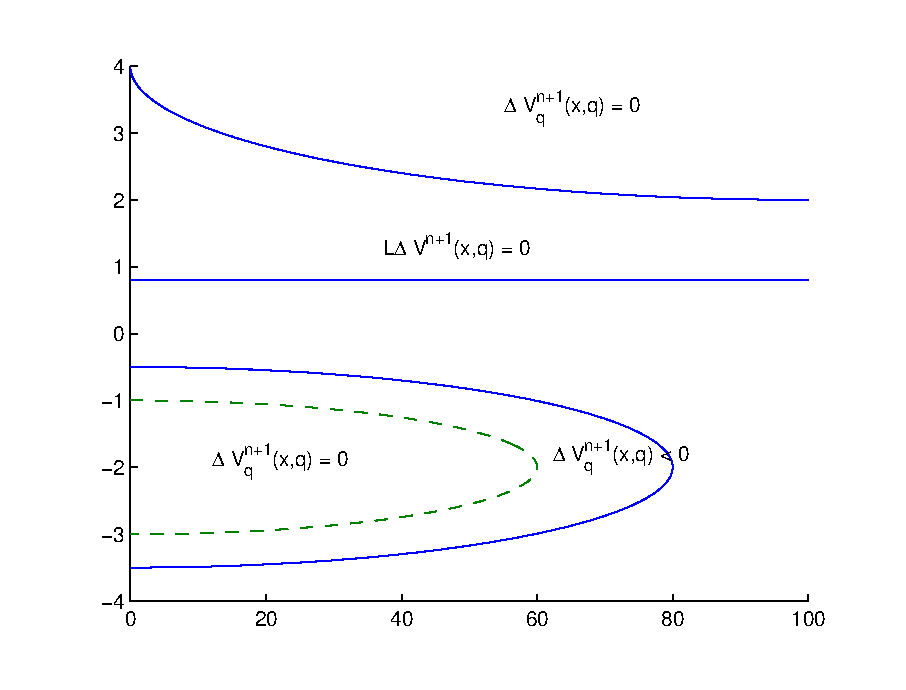
\includegraphics{deltaVstage2.eps}
  \caption{The equations that $\Delta V^{n+1}$ satisfies in the second stage.}
\end{figure}


Therefore we prove that we can continue moving the boundary.

 
\end{proof}



\section{The optimal policy will sell or buy(I need to prove that it is only sell that is possible) when the price is high enough. Namely, holding region always has a higher bound.}

% TODO I need to change this title.
In this section, we would like to prove that it is impossible to hold when the price is high enough. If not, $\exists M_0>\alpha, \q$ such that for any $x>M_0$,
\begin{equation*}
\begin{split}
V_q(x,\q) & \leq e^{x} + \lambda\\
\LL V(x,\q) &=  0\\
V_q(x,\q) &\geq e^{x} - \mu.\\
\end{split}
\end{equation*}
Take derivative with respect to $q$ to both sides of second equality,
\begin{equation*}
\begin{split}
V_q(x,\q) & \leq e^{x} + \lambda\\
\LL V_q(x,\q) &=  0\\
V_q(x,\q) &\geq e^{x} - \mu.\\
\end{split}
\end{equation*}
Define
\begin{equation}\label{h}
h(x) = V_q(x,\q) - (e^x -\mu).
\end{equation}
Therefore, $\forall x>M_0$
\begin{equation}\label{hin}
0\leq h(x) \leq \lambda + \mu.
\end{equation}
Substitute (\ref{h}) into $\LL V_q(x,\q) = 0$, 
\begin{equation}\label{hPDE}
\frac{1}{2}\sigma^2h''(x) + k(\alpha-x)h'(x) - \beta h = - \frac{1}{2}\sigma^2 e^x + k (x- \alpha)e^x + \beta(e^x - \mu).
\end{equation}
First, we would like to prove that $h'(x)$ must change sign on $[M_0,\infty)$. If not, assume $h'(x) \geq 0~ \forall x>M_0$, then by  (\ref{hin}) and (\ref{hPDE})
\begin{equation}\label{h''}
\frac{1}{2}\sigma^2h''(x)  \geq - \frac{1}{2}\sigma^2 e^x + k (x- \alpha)e^x + \beta(e^x - \mu).
\end{equation}
However, by Fubini's theorem, $\forall N > M_0$
\begin{equation}\label{Fubini}
\begin{split}
h(N) - h(M_0) &= \int_{M_0}^{N}h'(t)dt = \int_{M_0}^{N}(\int_{M_0}^{t}h''(x)dx+h'(M_0))dt\\
&=  \int_{M_0}^{N}\int_{M_0}^{t}h''(x)dxdt +(N-M_0)h'(M_0)\\
&= \int_{M_0}^{N}\int_{x}^{N}h''(x)dtdx +(N-M_0)h'(M_0)\\
&= \int_{M_0}^{N}(N-x)h''(x)dx +(N-M_0)h'(M_0).
\end{split}
\end{equation}
Substitute (\ref{h''}) and $h'(M_0) \geq 0$ into (\ref{Fubini})
\begin{equation*}
\begin{split}
h(N) - h(M_0)  &= \int_{M_0}^{N}(N-x)h''(x)dx +(N-M_0)h'(M_0)\\
&\geq  \int_{M_0}^{N}(N-x)(- e^x + \frac{2k}{\sigma^2} (x- \alpha)e^x + \frac{2\beta}{\sigma^2}(e^x - \mu))dx
\end{split}
\end{equation*}
which shows that $h(N) - h(M_0) \rightarrow +\infty$ when $N\rightarrow +\infty$. However via (\ref{hin}),
\begin{equation}\label{bound}
-(\lambda+\mu) \leq h(N)-h(M_0) \leq (\lambda + \mu)
\end{equation}  
holds when $\forall N >M_0$. Contradiction!\\
 Assume that $h'(x) < 0 ~\forall x>M_0$. Define
 \begin{equation*}
 g(x) = - \frac{1}{2}\sigma^2 e^x + k (x- \alpha)e^x + \beta(e^x - \mu) - k(x-\alpha).
 \end{equation*}
 Then we have
 \begin{equation*}
 g'(x) = - \frac{1}{2}\sigma^2 e^x + k (x- \alpha+1)e^x + \beta e^x  - k.
 \end{equation*}
 Noticing that both $g(x) \rightarrow +\infty$ and $g'(x) \rightarrow +\infty$ when $x \rightarrow +\infty$, there exists a $M_1 > M_0$ such that $g(M_1) > 0$ and $g(x)$ is increasing on $[M_1,+\infty)$. On the other hand, 
combining (\ref{bound}) and
 \begin{equation*}
 h(N) - h(M_1) = \int_{M_1}^{N} h'(t) dt,
 \end{equation*}
 there must exist a $M_2 > M_1$ which satisfies that $h'(M_2) > -1$. By (\ref{hPDE})
 \begin{equation*}
 \frac{1}{2}\sigma^2h''(M_2)  \geq - \frac{1}{2}\sigma^2 e^{M_2} + k (M_2- \alpha)e^{M_2} + \beta(e^{M_2} - \mu) - k({M_2}-\alpha) =g(M_2)>0
 \end{equation*}
 namely
 \begin{equation*}
 h''(M_2) > 0.
 \end{equation*}
 Let $\x = \inf\{x>M_2|h'(x) = -1\}$. If $\x < +\infty$ then $h''(\x) \leq 0$. However, (\ref{hPDE}) at point $\x$ shows us
 \begin{equation*} 
 \begin{split}
 \frac{1}{2}\sigma^2h''(\x) &= - \frac{1}{2}\sigma^2 e^{\x} + k (\x- \alpha)e^{\x} + \beta(e^{\x} - \mu) + k(\x-\alpha)h'(\x) + \beta h(\x)\\
&\geq - \frac{1}{2}\sigma^2 e^{\x} + k (\x- \alpha)e^{\x} + \beta(e^{\x} - \mu) - k(\x-\alpha) = g(\x).
 \end{split}
 \end{equation*}
 Since  $g(x)$ is increasing on $[M_1,+\infty)$, $g(\x) \geq g(M_1)  > 0$. 
 \begin{equation*}
  \frac{1}{2}\sigma^2h''(\x) = g(\x) > 0.
 \end{equation*}
 Contradiction! Therefore $h'(x)$ must change signs infinite times since we can replace $M_0$ with a sequence whose limit is $+\infty$.  Let $M_3$ be the point that $h'(x)$ changes from positive to negative. $M_3$ can be arbitrarily large and $h'(M_3) = 0$, $h''(M_3) \leq 0$. However, at point $M_3$ there is no chance that (\ref{hPDE}) holds when $M_3$ is large enough. Contradiction! We prove that we must inject or withdraw at some  prices. Section 1 shows that injection is impossible here, so we must withdraw at some prices.\\
 
 % todo Actually it is possible to quantify 'large enough' in this section. $x^*$ is big enough if expression $g(x)$ is positive when $x\geq x^*$.
 
 
\section{At optimal, buy and sell won't occur at the same price level.}

Assume \textbf{$V_{xxq}(x,q)$ exists in the holding region and $V_{xq}$ is continuous with respect to $q$ at the buying and selling boundaries.}\\

\begin{proof}
Assume $(x_0,q_0)$ is at the buying boundary and holding region is above it. 

\begin{equation}\label{eq1}
\begin{split}
V_q(x_0,q_0) &= e^{x_0} + \lambda(q_0)\\
V_{qx}(x_0,q_0) &= (e^{x}+\lambda(q_0))_x|_{x=x_0} = e^{x_0}\\
\LL V_q(x_0+,q_0) &= 0 \\ 
\end{split}
\end{equation}

Define
\begin{equation*}
f(x) = V_q(x,q_0) - (e^{x} + \lambda(q_0)).
\end{equation*}

We have 

\begin{equation}\label{eq2}
\begin{split}
f(x_0) &= V_q(x_0,q_0) - (e^{x_0} + \lambda(q_0)) = 0\\
f'(x_0) & = V_{qx}(x_0,q_0) - e^{x_0} = 0\\
\end{split}
\end{equation}

and 

\begin{equation}\label{eq3}
\LL f(x_0+) = \LL V_q(x_0+,q_0) - \LL(e^x + \lambda(q_0))|_{x=x_0} = - \LL(e^x + \lambda(q_0))|_{x=x_0}.
\end{equation}

On the other hand, for any point $(x,q)$ in the holding region

\begin{equation*}
\begin{split}
e^x - \mu(q) < V_q(x,q) < e^x + \lambda(q).
\end{split}
\end{equation*}

and at $(x_0,q_0)$ we have $V_q(x_0,q_0) = e^{x_0} + \lambda(q_0)$. These mean that $f(x)$ achieves its maximum at point $x_0$. Combined with (\ref{eq2}), $f''(x_0-) \leq 0$. Thus 
\begin{equation*}
\LL f(x_0+) = \frac{1}{2} \sigma^2 f''(x_0+) + k(\alpha- x_0)f'(x_0) -\beta f(x_0) = \frac{1}{2} \sigma^2 f''(x_0) \leq 0.
\end{equation*}

Then (\ref{eq3}) implies that  
\begin{equation*}
\begin{split}
-\LL(e^{x_0} +\lambda(q_0))&\leq 0  \\
- (\frac{1}{2} \sigma^2 e^{x_0} + k(\alpha -x_0) e^{x_0} - \beta (e^{x_0} +\lambda(q_0)))&\leq 0.
\end{split}
\end{equation*}

namely 
\begin{equation}\label{geqbuy}
\frac{1}{2} \sigma^2 e^{x_0} + k(\alpha -x_0) e^{x_0} - \beta (e^{x_0} +\lambda(q_0))) \geq 0.
\end{equation}


Noticing that above inequality holds no matter the holding boundary is below or above $(x_0,q_0)$.\\

Similarly, \textbf{if $(x_0,q_1)$ is at the selling boundary,} we have 

\begin{equation}\label{leqsell}
\frac{1}{2} \sigma^2 e^{x_0} + k(\alpha -x_0) e^{x_0} - \beta (e^{x_0} -\mu(q_1))) \leq 0.
\end{equation}

Since 
\[
\frac{1}{2} \sigma^2 e^{x_0} + k(\alpha -x_0) e^{x_0} - \beta (e^{x_0} -\mu(q_1))) > \frac{1}{2} \sigma^2 e^{x_0} + k(\alpha -x_0) e^{x_0} - \beta (e^{x_0} + \lambda(q_0)))  
\]
holds for any $q_1,q_2 \in [Q_{\min},Q_{\max}]$, it is impossible for (\ref{geqbuy}) and (\ref{leqsell}) hold at the same time. This is the same as saying that buy and sell won't occur at the same $x_0$.

\end{proof}


\newpage
\section{When futures are redundant?}


Let $F_{t,T}$ denote the price at time $t$ of future whose maturity is $T$. $Q,P$ are risk-neutral and historical measure respectively. If the prices are consistent with underlying asset price $exp(X_t)$, 

\begin{equation*}
 \exp(-\beta t) F_{t,T} = E_{Q} ( \exp(-\beta T)\exp(X_T) |\mathcal{F}_t)
\end{equation*}

The discounted profit of selling one unit commodity via this future is 

\begin{equation*}
\begin{split}
  &\exp(-\beta t) F_{t,T} - \exp(-\beta T) \int_{Q}^{Q+1}\mu(q) dq\\
  =&  E_{Q} ( \exp(-\beta T)\exp(X_T) |\mathcal{F}_t) - \exp(-\beta T) \int_{Q}^{Q+1}\mu(q) dq\\
  =&  E_{Q} ( \exp(-\beta T)\exp(X_T) - \exp(-\beta T) \int_{Q}^{Q+1}\mu(q) dq
   |\mathcal{F}_t).\\
   =&  E_{Q} ( e^{-\beta T}(e^{X_T} - \mu(Q^1_T)|\mathcal{F}_t).
\end{split}
\end{equation*}

where $\mu(Q^1_T) = \int_{Q}^{Q+1}\mu(q) dq$. 


Similarly total discounted cost of one unit commodity bought via this future is 

\begin{equation*}
\begin{split}
  &\exp(-\beta t) F_{t,T} + \exp(-\beta T) \int_{Q}^{Q+1}\lambda(q) dq\\
  =&  E_{Q} ( \exp(-\beta T)\exp(X_T) |\mathcal{F}_t) + \exp(-\beta T) \int_{Q}^{Q+1}\lambda(q) dq\\
  =&  E_{Q} ( \exp(-\beta T)\exp(X_T) + \exp(-\beta T) \int_{Q}^{Q+1}\lambda(q) dq
   |\mathcal{F}_t)\\
   =&  E_{Q} ( e^{-\beta T}(e^{X_T} + \lambda(Q^2_T)|\mathcal{F}_t). 
\end{split}
\end{equation*}
where $\lambda(Q^2_T) = \int_{Q}^{Q+1}\lambda(q) dq)$.


Recall the objective function without futures.

\begin{equation}
  V(x,q) = \max_{(L,U) \in \mathcal{U}} \mathbb{E}_P \left(\int_{0}^{\infty} e^{-\beta t}(e^{X_t} - \mu(Q^1_t))dU_t - \int_{0}^{\infty}e^{-\beta t}(e^{X_t} + \lambda(Q^2_t))dL_t\right)
\end{equation}

Notice, this expectation is under historical measure. If $P = Q$, the future is redundant. If $P \neq Q$, it is not.

%Assume we also have another boundary point with the same level of price on the left hand side of $(x_0,q_0)$ , i.e. $(x_0,q_1)$ where $q_1 < q_0$ and there is no other boundary point between them. Therefore
%
%\begin{equation*}
%\begin{split}
%V(x_0,q_0) &= V(x_0,q_1) + \int_{q_1}^{q_0} V_q(x_0,q) dq\\
%&=V(x_0,q_1) + (q_1-q_0) e^{x_0} + \int_{q_1}^{q_0} \lambda(q) dq.
%\end{split}
%\end{equation*}
%
%Use operator $\LL$ to both sides, 
%
%\begin{equation*}
%\LL V(x_0,q_0) = \LL V(x_0,q_1) + \LL ((q_1-q_0) e^{x_0} + \int_{q_1}^{q_0} \lambda(q) dq)
%\end{equation*}
%
%By the continuity of $V_{xx}, V_{x}, V$  with respect to $q$ on the boundary, we have 
%
%\begin{equation*}
%\LL V(x_0,q_0) = \LL V(x_0,q_1) = 0.
%\end{equation*}
%
%So
%\begin{equation*}
%\LL ((q_1-q_0) e^{x_0} + \int_{q_1}^{q_0} \lambda(q) dq) = 0,
%\end{equation*}
%
%which gives us
%
%\begin{equation*}
%\frac{1}{2} \sigma^2 e^{x_0} + k(\alpha -x_0) e^{x_0} - \beta (e^{x_0} +\frac{1}{q_0-q_1}\int_{q_1}^{q_0}\lambda(q)dq) = 0.
%\end{equation*}
%
%This can't happen if $\lambda(q)$ is strictly increasing on $[q_1,q_0]$, because by (\ref{geq})
%
%\begin{equation*}
%\begin{split}
%\frac{1}{2} \sigma^2 e^{x_0} + k(\alpha -x_0) e^{x_0} - \beta e^{x_0} \geq \beta \lambda(q_0) >\frac{1}{q_0-q_1}\int_{q_1}^{q_0}\lambda(q)dq .
%\end{split}
%\end{equation*}
%
%Assume that there is another boundary point $(x_0,q_2)$ at the right hand side of $(x_0,q_0)$, namely $q_2>q_0$ and the region between them are holding region. By the previous result, there can't be a boundary point on the right hand side of $(x_0,q_2)$. Let $(x_0,q_3)$ where $q_3 > q_2$, then $(x_0,q_3)$ must belong to injection region.
%
%Similarly
%
%\begin{equation*}
%\begin{split}
%\LL V(x_0,q_2) &= 0 \\
%\LL V(x_0,q_3)& < 0\\
%V(x_0,q_3) &= V(x_0,q_2) + (q_3-q_2) e^{x_0} + \int_{q_2}^{q_3} \lambda(q) dq.
%\end{split}
%\end{equation*}
% 
%Use operator $\LL$ to both sides of the last equality and use the top two 
%
%\begin{equation*}
%0>\LL V(x_0,q_3) = 0 + (q_3-q_2) (\frac{1}{2} \sigma^2 e^{x_0} + k(\alpha -x_0) e^{x_0} - \beta (e^{x_0} +\frac{1}{q_3-q_2}\int_{q_2}^{q_3}\lambda(q)dq)).
%\end{equation*}
%
%This shows that 
%
%\begin{equation*}
% \frac{1}{2} \sigma^2 e^{x_0} + k(\alpha -x_0) e^{x_0} - \beta (e^{x_0} +\frac{1}{q_3-q_2}\int_{q_2}^{q_3}\lambda(q)dq) < 0.
%\end{equation*}
%
%Let $q_3 \rightarrow q_2$, 
%
%\begin{equation*}
% \frac{1}{2} \sigma^2 e^{x_0} + k(\alpha -x_0) e^{x_0} - \beta (e^{x_0} +\lambda(q_2) )\leq 0.
%\end{equation*}
%
%On the other hand, $(x_0,q_2)$ is the boundary point, thus
%
%\begin{equation*}
% \frac{1}{2} \sigma^2 e^{x_0} + k(\alpha -x_0) e^{x_0} - \beta (e^{x_0} +\lambda(q_2) )\geq 0.
%\end{equation*}
%
%Combine those two,
%
%\begin{equation*}
%\frac{1}{2} \sigma^2 e^{x_0} + k(\alpha -x_0) e^{x_0} - \beta (e^{x_0} +\lambda(q_2) )= 0.
%\end{equation*}
%
%



 
 %%%%%%% This part is wrong %%%%%%%%%%%%
% \section{Withdraw region}
% In this section we would like to show that if $(M, \q)$ is a withdrawing point and $M$ is big enough, any point $(x,\q)$ where $x>M$ is also a withdrawing point. If not, let $(x_3,\q)$ be the point changes from withdrawal to holding. The smooth fit conditions tell us
% \begin{equation*}
% h(x_3) = 0 \quad h'(x_3) =0
% \end{equation*}
% where $h(x)$ is defined in the previous section. Define
% \begin{equation*}
% x_4 = \inf\{x>x_3|h'(x)=0\}.
% \end{equation*}
%If $x_4 < +\infty$, 
%\begin{equation*}
%h'(x_4) =0 \quad h''(x_4) \leq 0 .
%\end{equation*}
%However, it is impossible to have (\ref{hPDE}) hold at point $x_4$ when $x_4$ is big enough. Thus $x_4 = +\infty$ namely $h'(x) > 0~ \forall x > x_3$. On the other hand, previous section tells us there must be another withdrawing point $x_5 > x_3$. Still by smooth fit conditions at $x_5$, $h'(x_5) = 0$. Contradiction! \\
%
%Actually it is possible to quantify 'big enough' in this section. $x^*$ is big enough if expression $
%- \frac{1}{2}\sigma^2 e^x + k (x- \alpha)e^x + \beta(e^x - \mu)$ is positive when $x\geq x^*$.
%I want to show that it is impossible to inject when the price is big enough. And amazingly I should that it is impossible to change from holding to injection. First recall the PDE we have.
%\begin{equation}
%\frac{1}{2}\sigma^2f''(x) + k(\alpha-x)f'(x) - \beta f(x) = - \frac{1}{2}\sigma^2 e^x + k(x-\alpha)e^x + \beta(e^x - \mu) 
%\end{equation}
%At the injection point $x_0$, we have $f(x_0) = \mu + \lambda$ and $f'(x_0) = 0$. If we approach $x_0$ from holding region we should have\footnote{$f''$ is not continuous at point $x_0$.}
%\begin{equation}
%\frac{1}{2}\sigma^2f''(x_0) - \beta (\mu+\lambda)= - \frac{1}{2}\sigma^2 e^{x_0} + k(x_0-\alpha)e^{x_0} + \beta(e^{x_0} - \mu) 
%\end{equation}
%Therefore,
%\begin{equation}
%\frac{1}{2}\sigma^2f''(x_0)= - \frac{1}{2}\sigma^2 e^{x_0} + k(x_0-\alpha)e^{x_0} + \beta(e^{x_0} + \lambda)
%\end{equation}
%Let 
%\begin{equation}
%t(x) =  - \frac{1}{2}\sigma^2 e^{x} + k(x-\alpha)e^{x} + \beta(e^{x} + \lambda)
%\end{equation}
%If  $t(x_0) > 0$ then $f''(x_0) > 0$. However, $f$ has the maximum value as $\mu + \lambda$ and $f'(x_0) = 0$, therefore $f''(x_0) \leq0$. Contradiction. Therefore, we must have $t(x_0) \leq 0$.  Then $f(x) = \mu + \lambda~for ~\{x>x_0\}\cap\{injection~region\} $. If we approach $x_0$ from above we should have 
%\begin{equation}
%\frac{1}{2}\sigma^2f''(x_0) + k(\alpha-x_0)f'(x_0) - \beta f(x_0) < - \frac{1}{2}\sigma^2 e^{x_0} + k(x_0-\alpha)e^{x_0} + \beta(e^{x_0} - \mu)
%\end{equation}
%\begin{equation}
%- \beta (\mu+\lambda) < - \frac{1}{2}\sigma^2 e^{x_0} + k(x_0-\alpha)e^{x_0} + \beta(e^{x_0} - \mu)
%\end{equation}
%\begin{equation}
%0 < - \frac{1}{2}\sigma^2 e^{x_0} + k(x_0-\alpha)e^{x_0} + \beta(e^{x_0} + \lambda) = t(x_0)
%\end{equation}
%Contradiction!
%
%Next I want to show when the price is low enough we always inject!
%It is easy to show that it is impossible to withdraw when the price is low enough since the \limits PDE left = 0 ,right < 0 which contradicts the definition of withdraw region.
% 
%
%\section*{Conclusion}
%
%\bibliographystyle{unsrt}
%
%\bibliography{sample}
%
%----------------------------------------------------------------------------------------
%
\end{document}